\chapter{Luca}

\begin{enumerate}
  \item \sd, go right and up to the next screen, \cs[2:30]. Don't save.
  \item \sd\ in locker room. Don't do the tutorial. \sd, walk down, \sd
  \item Walk down to next screen, \sd. Whistle \cs[0:30], walk right to next screen.
  \item \sd, run to the cafe. \sd, \skippablefmv+\cs[1:20], \sd
  \item Run left to next screen, then left to the docks. Run north to the next screen.
\end{enumerate}
\begin{battle}{Machina}
  \begin{itemize}
    \item \textit{For the first two encounters:}
          \begin{itemize}
            \tidusf Defend
            \kimahrif Defend
            \luluf Thunder
          \end{itemize}
    \item \textit{For the third encounter:}
          \begin{itemize}
            \item \textit{First Wave}
                  \begin{itemize}
                    \tidusf Attack
                    \kimahrif Attack
                    \luluf Thunder a different Machina
                    \tidusf Attack
                    \kimahrif \od\ Seed Cannon \textit{if no crits else} Attack
                  \end{itemize}
            \item \textit{Second Wave}
                  \begin{itemize}
                    \tidusf Defend
                    \kimahrif Defend
                    \luluf Thunder
                  \end{itemize}
            \item \textit{Third Wave}
                  \begin{itemize}
                    \tidusf Attack
                    \kimahrif Attack
                    \luluf Thunder a different Machina
                  \end{itemize}
          \end{itemize}
  \end{itemize}
\end{battle}
\begin{enumerate}[resume]
  \item If anyone is Critical HP, use Potions.
  \item Run right.
\end{enumerate}
\begin{battle}[3000]{Oblitzerator}
  \begin{itemize}
    \kimahrif Defend
    \tidusf Defend
    \luluf Thunder Crane x3
    \tidusf Use Crane after \lulu's string
    \kimahrif Defend
    \luluf Thunder
    \tidusf Defend
  \end{itemize}
  Check for \textbf{Lightning Steel, Thunder Ball}
\end{battle}
\begin{enumerate}[resume]
  \item \cs[2:00], \sd\ during and after Blitzball game.
\end{enumerate}
\vfill
\begin{spheregrid}
  \begin{itemize}
    \tidusf Jump straight to Str Node
    \tidusf +1 Str, Haste, +20 MP
  \end{itemize}
  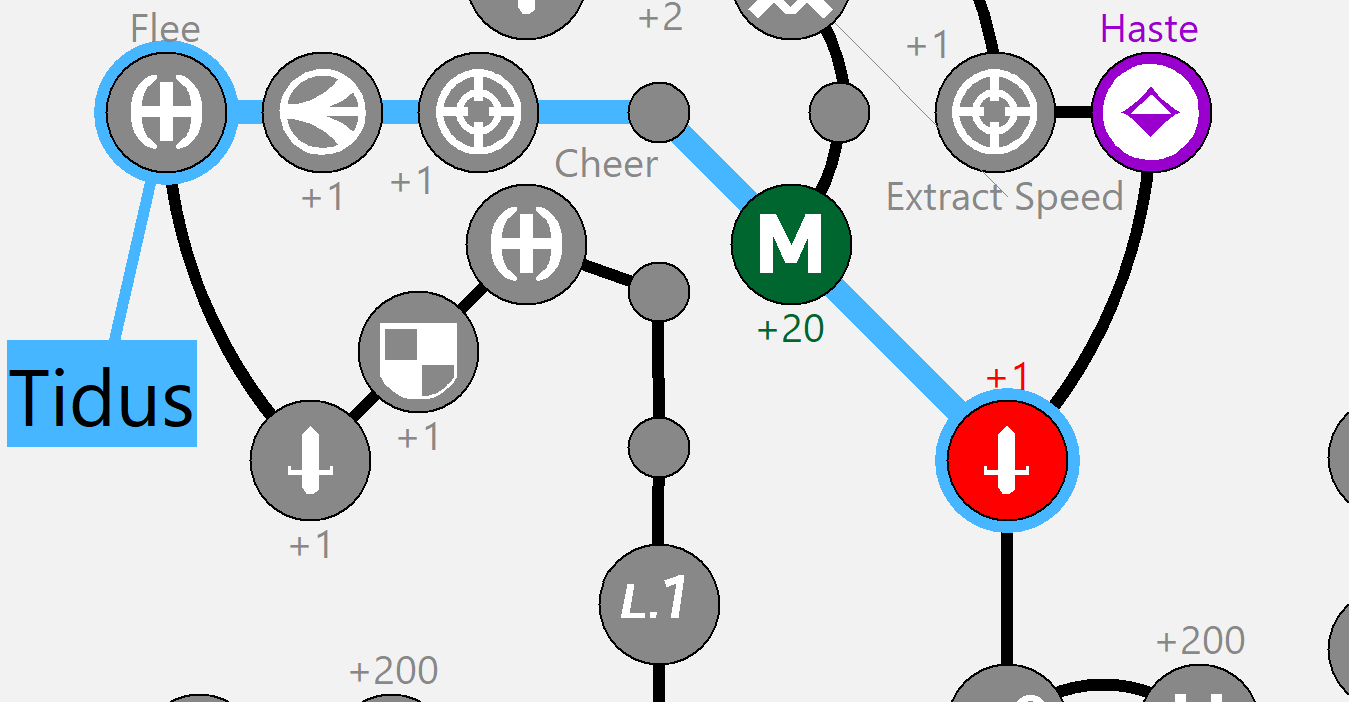
\includegraphics{graphics/haste}
\end{spheregrid}
\begin{equip}
  \begin{itemize}
    \item \textit{If you got Lightning Steel}
          \begin{itemize}
            \tidusf Equip Lightning Steel
          \end{itemize}
  \end{itemize}
\end{equip}
\begin{enumerate}[resume]
  \item Auto-Sort items
  \item Run South for the next two screens. \save. Go up the stairs to the locker room, \sd
  \item Go back into locker room, speak to \wakka, \sd, \cs[1:20]. \sd\ after \lulu\ scene. \cs[1:40] on Auron Entrance.
\end{enumerate}
\begin{trial}
  \textbf{Blitzball}
  \begin{itemize}
    \item \textit{If Luca wins the Blitzoff:}
          \begin{itemize}
            \item Triangle, switch the mode to \textbf{Mark Mode}
            \item When Graav is close to your central player, return to \textbf{Normal Mode}
          \end{itemize}
    \item \textit{When you get the ball:}
          \begin{itemize}
            \item Change to \textbf{Manual A} and \textbf{Normal Mode}
            \item Hide behind the Goalie
            \item Alternatively pass to Jassu and swim around
            \item Only try to score when the time is almost up
            \item If losing, don't try to score
          \end{itemize}
    \item \sd\ during half time, \sd\ during \wakka\ protest, \sd\ end of game.
  \end{itemize}
\end{trial}
\begin{enumerate}[resume]
  \item \cs[1:00], Don't Save
\end{enumerate}
\begin{battle}{Sahagin Chief}
  \begin{itemize}
    \item{If no Lightning Steel:}
          \begin{itemize}
            \tidusf Haste \tidus
            \wakkaf Attack one Sahagin for the first two waves, defend on the third wave
            \tidusf Attack the other Sahagin
            \wakkaf Potion if \tidus\ has less than 150 HP
          \end{itemize}
    \item{If Lightning Steel:}
          \begin{itemize}
            \tidusf Haste \tidus
            \tidusf Cheer x2
            \wakkaf Attack
            \tidusf Attack
          \end{itemize}
  \end{itemize}
\end{battle}
\begin{enumerate}[resume]
  \item \sd, \skippablefmv
\end{enumerate}
\begin{battle}[1800]{Garuda}
  \begin{itemize}
    \tidusf Haste \auron
    \auronf Attack x3
    \wakkaf Defend
    \tidusf Defend until \auron\ finishes his string, then Attack
    \auronf Attack x3
    \item Don't revive non-\auron\ party members
  \end{itemize}
\end{battle}
\begin{enumerate}[resume]
  \item \cs+\skippablefmv[1:30]. Don't save. \sd\ the Auroch scene
  \item \cs[4:50]. Run north to the hidden chests, \pickup{Magic and HP Sphere}
  \item Run South and try to speak to \auron\ while he's walking away.
  \item Follow red arrow to \yuna. \sd\ during guardian scene. Walk to \yuna, \cs[4:20]
\end{enumerate}